\documentclass[a4paper]{jpconf}
\usepackage{graphicx}

% Packages physics of fluids 
\usepackage{tabularx}
\usepackage{multirow}

\usepackage{booktabs,caption,fixltx2e}
\usepackage[flushleft]{threeparttable}


\usepackage{arydshln}

% Packages philtrans
\usepackage{mathrsfs}
\usepackage{amsmath}
\usepackage{amsfonts}
\usepackage{epstopdf}
\usepackage{etoolbox}
\usepackage{tikz}
\usepackage[outline]{contour}
\newcommand{\addref}{{\color{blue} REF}}
\newcommand{\ufilt}{\tilde{\boldsymbol{u}}}
\newcommand{\commwim}[1]{{\color{red} #1}}
\newcommand{\dx}{\text{d}\boldsymbol{x}}
\newcommand{\dt}{\text{d}t}
\newcommand{\ddd}{\text{d}}
\newcommand{\ddt}[1]{\frac{\ddd #1}{\ddd t}}
\newcommand{\blds}[1]{\boldsymbol{#1}}
\newcommand{\dd}[2]{\frac{\ddd #1}{\ddd #2}}
\newcommand{\ctihat}{\widehat{C}_{T,i}'}
\newcommand{\cthat}{\widehat{C}_T'}
\newcommand{\ctmax}{C_{T,\text{max}}'}

\newcommand{\legend}{(\emph{Legend}: R: {\bf \color{black}-----}, C3t0: {\bf \color{red}-----}, C3t5: {\bf\color{Dandelion}-----}, C3t30: {\bf\color{Cyan}-----}, C2t0: {\bf\color{red}- - -}, C2t5: {\bf\color{Dandelion}- - -}, C2t30: {\bf\color{Cyan}- - -})}
\newcommand{\legendtauref}{(\emph{Legend}: R: {\bf \color{black}-----}, $\tau = 0$ s: {\bf \color{red}-----}, $\tau = 5$ s: {\bf\color{Dandelion}-----}, $\tau = 30$ s: {\bf\color{Cyan}-----})}

\newcommand{\legendnoref}{C3t0: {\bf \color{red}-----}, C3t5: {\bf\color{Dandelion}-----}, C3t30: {\bf\color{Cyan}-----}, C2t0: {\bf\color{red}- - -}, C2t5: {\bf\color{Dandelion}- - -}, C2t30: {\bf\color{Cyan}- - -}}

\newcommand{\legendtau}{(\emph{Legend}: $\tau = 0$ s: \contour{red}{\color{red}-----}, $\tau = 5$ s: \contour{Dandelion}{\color{Dandelion}-----}, $\tau = 30$ s: \contour{Cyan}{\color{Cyan}-----})}
%\newcommand{\legendtauref}{(\emph{Legend}: R: \contour{black}{\color{black}-----}, $\tau = 0$ s: \contour{red}{\color{red}-----}, $\tau = 5$ s: \contour{Dandelion}{\color{Dandelion}-----}, $\tau = 30$ s: \contour{Cyan}{\color{Cyan}-----})}

\newrobustcmd*{\mycircle}[1]{\tikz{\filldraw[draw=#1,fill=#1] (0,0) 
		circle [radius=0.08cm];}}
\newrobustcmd*{\mycircleopen}[1]{\tikz{\filldraw[draw=#1,fill=white] (0,0) circle [radius=0.08cm];}}

% Yawing paper
% Additional packages to be loaded
%---------------------------------------------------------------------------------
\usepackage{mathtools}
\usepackage{mathrsfs}
\usepackage{amsmath}
\usepackage[short]{optidef}
\usepackage{printlen}
\usepackage{tikz}
\usepackage{xcolor}

\definecolor{C1}{RGB}{31,119,180}
\definecolor{C2}{RGB}{255,127,14}
\definecolor{C3}{RGB}{44,160,44}
\definecolor{C4}{RGB}{214,39,40}

% Some  auxiliary commands for ease of mathematics notations
%---------------------------------------------------------------------------------
% Derivatives and differentials
\newcommand{\ds}{~\text{d}\boldsymbol{s}}
\newcommand{\dzeta}{~\text{d}\boldsymbol{\zeta}}
\newcommand{\pder}[2]{\frac{\partial #1}{\partial #2}}
\newcommand{\bolds}[1]{\boldsymbol{#1}}
% Integrals
\newcommand{\stint}{\int_{0}^{T} \int_{\Omega}}
\newcommand{\sint}{\int_{\Omega}}
\newcommand{\Tint}{\int_{0}^{T}}
\newcommand{\tint}{\int_{0}^{t}}
% Filtered variables
\newcommand{\utilde}{\widetilde{\bolds{u}}}
\newcommand{\ptilde}{\widetilde{p}}
\newcommand{\ctnhat}[1]{\widehat{C}_{T,#1}'}
% Other symbols
\newcommand{\cti}{C_{T,i}'}
\newcommand{\ctn}[1]{C_{T,#1}'}
\newcommand{\R}{\mathscr{R}}
\newcommand{\J}{\mathscr{J}}
\newcommand{\Jtilde}{\tilde{\mathscr{J}}}
\newcommand{\Jgrad}{\nabla \Jtilde}
\newcommand{\Lagr}{\mathscr{L}}
\newcommand{\eperp}{\bolds{e}_\perp}
\newcommand{\eperpi}{\bolds{e}_{\perp,i}}
\newcommand{\etransi}{\bolds{e}_{\parallel,i}}
\newcommand{\ex}{\bolds{e}_x}
\newcommand{\ey}{\bolds{e}_y}
\newcommand{\ez}{\bolds{e}_z}
\newcommand{\eperpn}[1]{\bolds{e}_{\perp,#1}}
\newcommand{\vi}{\frac{1}{A_i} \sint \R_i (\bolds{s})~\utilde \cdot \eperpi \ds}
% Operators
\newcommand{\innerproduct}[2]{\bigg( #1, #2 \bigg)}
\newcommand{\innerproductsmall}[2]{\big( #1, #2 \big)}
\newcommand{\sumturbines}{\sum_{i=1}^{N_t}}
\newcommand{\diracdelta}{{\delta}}
% Colors
\newcommand{\red}[1]{{\color{red} #1}}
\newcommand{\purp}[1]{{\color{purple} #1}}
\newcommand{\reftodo}[1]{\red{AddREF}: #1}
\newcommand{\todo}[1]{\purp{TODO: #1}}
\newcommand{\fixeqref}{\purp{FixEqRef}}
%---------------------------------------------------------------------------------

%---------------------------------------------------------------------------------
\usepackage{mathtools}
\usepackage{mathrsfs}
\usepackage{amsmath}
\usepackage[short]{optidef}
\usepackage{printlen}
\usepackage{tikz}
\usepackage{xcolor}

\definecolor{C1}{RGB}{31,119,180}
\definecolor{C2}{RGB}{255,127,14}
\definecolor{C3}{RGB}{44,160,44}
\definecolor{C4}{RGB}{214,39,40}
\DeclareMathOperator*{\argmin}{arg\,min}

\newcommand{\sqdiamond}[1][fill=gray]{\tikz [x=1.2ex,y=1.85ex,line width=.1ex,line join=round, yshift=-0.285ex] \draw  [#1]  (0,.5) -- (.5,1) -- (1,.5) -- (.5,0) -- (0,.5) -- cycle;}%
\newcommand{\miDiamond}[1][fill=gray]{\mathop{\raisebox{-0.275ex}{$\sqdiamond[#1]$}}}



\begin{document}
\title{Optimal dynamic induction and yaw control of wind farms: effects of turbine spacing and layout}

\author{Wim Munters and Johan Meyers}

\address{Department of Mechanical Engineering, KU Leuven, Celestijnenlaan 300A, B3001 Leuven, Belgium}

\ead{wim.munters@kuleuven.be, johan.meyers@kuleuven.be}

\begin{abstract}
Turbine wake interactions in wind farms result in decreased power extraction in downstream rows. The current work investigates dynamic induction and yaw control of wind farms for increased total power extraction. Six different wind farm layouts are considered, and the relative benefits of induction control, yaw control, and combined induction--yaw control are compared. It is found that optimal control significantly increases wind-farm efficiency for virtually all cases, and that the most profitable control strategy between exclusive yaw and induction control depends on the effective wind-farm layout as seen by the flow, and hence the mean wind direction. 
\end{abstract}

\section{Introduction}
Turbine wake interactions in wind farms result in decreased power extraction in downstream rows. The promise of increasing total power extraction
through coordinated wind-farm control has incited a multitude of studies into axial induction control and yaw control of wind turbines. In earlier
work \cite{goit, munters}, a dynamic induction control approach was introduced based on large-eddy simulations (LES)  and optimization, and analysis of the optimization results led to the identification of a sinusoidal induction control strategy for first-row turbines \cite{munterswes}. Recently, the dynamic optimal control approach was expanded to also include yaw \cite{muntersenergies}. A control study of a $4 \times 4$ wind farm with 6 rotor diameters spacing illustrated that yaw control tends to be more favorable than induction control for small sets of aligned wind turbines, and that combining yaw and induction control potentially further increases power gains. 

In the current work, we aim to quantify and compare the potential power gains for induction control, yaw control and combined induction--yaw control in large wind farms with both aligned and staggered layouts. Especially in the latter, the abovementioned advantage of yaw control over induction control is expected to be diminished, since yaw could lead to detrimental interactions between different columns of wind turbines by transversally deflected turbine wakes. Control studies are performed for wind farms with the aforementioned 6 rotor diameter spacing between turbines as well as wind farms with an increased turbine density, where the effect of turbine wake interactions on wind-farm power is further increased.  

The paper is structured as follows. Firstly, Section \ref{sec:meth} elaborates on the optimal control methodology used in this study. Next, Section \ref{sec:setup} details the case setup. Subsequently, Section \ref{sec:results} presents the results of the optimization cases. Finally, Section \ref{sec:conc} formulates general conclusions and provides
suggestions for further research. 

 \section{Methodology} \label{sec:meth}

This section provides a brief description of the optimal control methodology used in the current paper. A more detailed description of the
methodology can be found in Refs. \cite{goit, munters, muntersenergies}. Figure \ref{fig:meth} provides a general overview of the methodology. Figure
\ref{fig:meth}a illustrates the control block diagram: the wind-farm control vector $\blds{\varphi}(t)$ is optimized until a set of optimal control
$\blds{\varphi}^{\bullet}(t)$ is found. The wind-farm flow model consists of a turbulence-resolving LES and the gradient of the 
cost functional $\J$ (i.e. the total wind-farm power) is evaluated using the continuous adjoint formulation of the LES system. In this way,
\emph{a priori} simplification of the representation of the boundary layer and turbine wakes are avoided as much as possible, and control signals can
be designed to tap into the unsteady dynamics of the turbulent flow.

\begin{figure}
	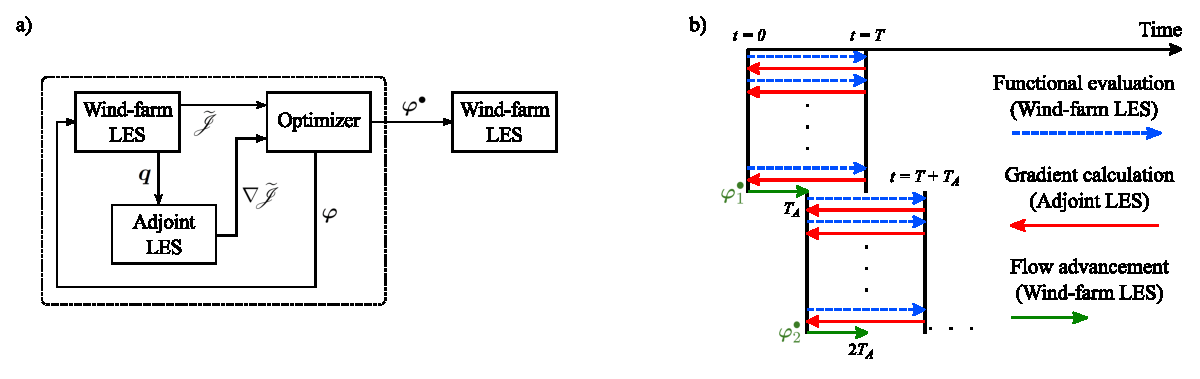
\includegraphics[width=\textwidth]{Torque18/figure1}
	\caption{Schematic overview of wind-farm optimal control methodology. \emph{a)} Control block diagram with adjoint gradient-based optimization
	and LES flow models illustrating data flow of (optimal) controls $\boldsymbol{\varphi}^{(\bullet)}$, system state $\boldsymbol{q}$, cost
	functional $\mathscr{J}$ and its gradient $\nabla \mathscr{J}$. \emph{b)} Receding horizon framework subdividing time into discrete flow
	advancement windows of length $T_A$ with prediction horizon $T$. Each arrow represents a forward or adjoint LES. Every window consists of an
	optimization stage (blue and red lines) follow by a flow advancement stage with optimal controls $\boldsymbol{\varphi}^{\bullet}$ (green
	lines). Figure adapted from Ref. \cite{munterswes} (published under a CC BY-4.0 license). \label{fig:meth} }
\end{figure}

Figure \ref{fig:meth}b illustrates the receding-horizon approach to wind-farm control followed in the current work. Wind-farm controls
are optimized over a finite time horizon $T$, resulting in a number of alternating LES and adjoint LES simulations, after which the
optimized controls $\blds{\varphi}^{\bullet}(t)$ are used in a flow advancement simulation with time horizon $T_A$. Within each window, wind-farm
operation is optimized by solving the following constrained optimization problem:  

\begin{alignat}{4}
& \underset{\bolds{\varphi}, \bolds{q}}{\text{min}}  & \qquad  \J(\bolds{\varphi}, \bolds{q}) &= - \Tint \sum_{i=1}^{N_t} \frac{1}{2} \ctihat~V_i^3 A_i \dt  & \label{eq:costfunction}\\
& \text{s.t.}                      			&         \frac{\partial \utilde}{\partial t} + \big(\utilde \cdot \nabla \big)~ \utilde &= - \nabla (\ptilde + \ptilde_\infty) / \rho - \nabla \cdot \boldsymbol{\tau}_{sgs} + \sum_{i=1}^{N_t} \bolds{f}_i \qquad  & \text{in } \Omega \times (0,T], \label{eq:NSmomentum_constraint} \\
&                                                   &        \nabla \cdot \utilde&=0 									        & \text{in } \Omega \times (0,T], \label{eq:NScontinuity_constraint}\\
&                                                   &        \tau \ddt{\ctihat}&=\cti - \ctihat 								& i=1\dots N_t~\text{in } (0,T],  \label{eq:ctihat_constraint}\\
&                                                   &        \ddt{\theta_i}&=\omega_i											& i=1\dots N_t~\text{in } (0,T],  \label{eq:omega_constraint}\\
&                                                   &        C_{T,\text{min}}' \leq~ &\cti \leq C_{T,\text{max}}'				& i=1\dots N_t~\text{in } (0,T],  \label{eq:boxct_constraint}\\
&                                                   &        -\omega_{\text{max}} \leq~ &\omega_i \leq \omega_{\text{max}}.   	& i=1\dots N_t~\text{in } (0,T],  \label{eq:boxomega_constraint}
\end{alignat}
with system states $\bolds{q}(\bolds{x},t) = [\ufilt(\bolds{x},t),\ \ptilde(\bolds{x},t),\ \ctnhat{1}(t), \dots, \ctnhat{N_t}(t), \theta_1(t), \dots,
\theta_{N_t}(t)]$ and controls $\bolds{\varphi}(t)~=~[\ctn{1}(t), \dots, \ctn{N_t}(t), \omega_1(t), \dots, \omega_{N_t}(t)]$. State equations
(\ref{eq:NSmomentum_constraint} -- \ref{eq:NScontinuity_constraint}) are the filtered Navier--Stokes equations modeling the turbulent wind-farm
boundary layer, which are discretized with a mixed spectral--finite difference method in space and a fourth order explicit Runge Kutta scheme in time. 
In these equations, $\ufilt$ and $\ptilde$ are the filtered velocity and pressure respectively. Further, $\nabla \ptilde_\infty$ is the driving background pressure gradient and $\bolds{\tau}_{\rm sgs}$ is the subgrid-scale stress tensor. The thrust force $\bolds{f}_i$ enacted on the flow by each turbine $i$ is modeled using an actuator disk approach as 
%\begin{equation}
$\bolds{f}_i = \frac{1}{2} \ctihat V_i^2 \R_i \eperpi$,
%\end{equation}
with $\ctihat$ the thrust coefficient, $\R_i$ the geometric footprint of the turbine on the LES grid, and $V_i = (1/A_i) \sint \R_i \utilde \cdot \eperpi \dx$ the disk-averaged velocity. The rotor-perpendicular vector $\eperpi = \bolds{e}_x \cos \theta_i + \bolds{e}_y \sin \theta_i$, with $\theta_i$ the turbine yaw angle. 
The thrust coefficient $\ctihat$ is obtained from its setpoint value $\cti$ through an exponential time filter with characteristic turbine response time $\tau = 5$ s (Eq. \ref{eq:ctihat_constraint}), and the turbine yaw angle is found through integration of the yaw rate $\omega_i$ (Eq. \ref{eq:omega_constraint}). Finally, controls are bound to technical box constraints in Eqs. (\ref{eq:boxct_constraint} - \ref{eq:boxomega_constraint}).
The optimization problem is solved in a reduced formulation using the gradient-based {L--BFGS--B} algorithm \cite{byrd}. As mentioned above, the cost functional gradient is calculated using the continuous adjoint method. A detailed elaboration of the adjoint equations and verification of the adjoint gradient is included in Ref. \cite{muntersenergies}, and is omitted here for brevity. 

\section{Case Setup}\label{sec:setup}
We consider a total of six wind farms, comprised of three layouts with two different spacings. Figure \ref{fig:wf_layouts} illustrates the wind farms
for the aligned ($A$), two-row staggered ($St2$), and three-row staggered ($St3$) cases. For each of these layouts, a tight (T) spacing and wide (W)
spacing arrangement is considered, with axial and transversal spacings of $S_T = 3.6D$ and $S_W = 6D$ respectively. The tightly and widely spaced
farms are simulated with a resolution of $26 \times 14 \times 6.9$ m$^3$ on domains of size $10 \times 3.6 \times 1$ km$^3$ and $7.5 \times 3.6 \times 1$ km$^3$,
hence resulting in simulation grids of $384 \times 256 \times 144$ and $288 \times 256 \times 144$ respectively in axial, transversal and vertical
directions. Inflow conditions are the same for all simulation cases and are generated in a separate precursor domain with shifted periodic boundary
conditions \cite{muntersshift} in which a driving pressure gradient of $\nabla \ptilde_\infty / \rho = 2.5 \times 10^{-4}$ m s$^{-2}$ results in a
free-stream velocity $U_\infty \approx 8.5 $ m s$^{-1}$ at hub height. Simulations are advanced in time with a constant timestep of $\Delta t = 0.75$ s. 

\begin{figure}
	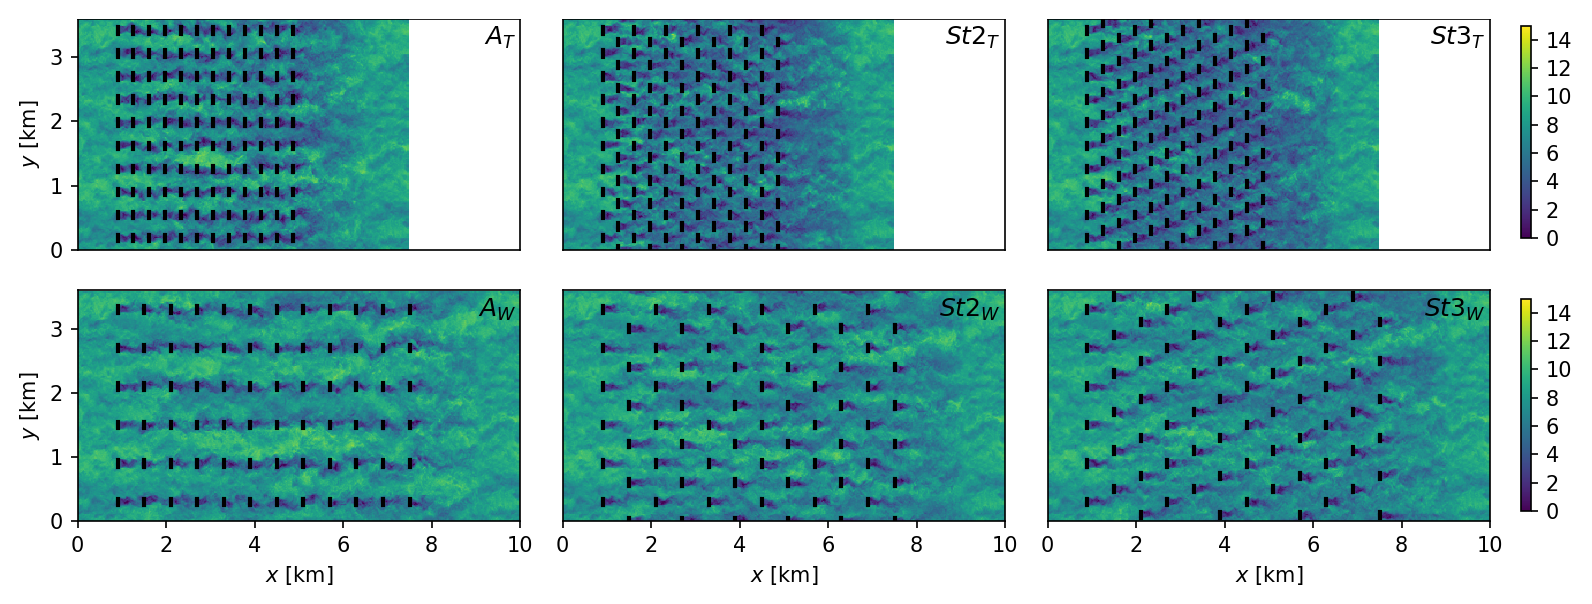
\includegraphics[width=\textwidth]{Torque18/eps/drawing.eps}
	\caption{Wind-farm layouts: (A) Aligned, (St2) Staggered every two rows, (St3) Staggered every three rows. Top: (T) Tight spacing, $S= 3.6D$. Bottom: (W) Wide spacing, $S = 6D$. Colors represent instantaneous streamwise velocity in m s$^{-1}$.\label{fig:wf_layouts}}
\end{figure}


For each farm, four control cases are considered. Firstly, a greedy reference control case (R) is defined, in which turbines have a yaw angle fixed perpendicular to
the mean-flow direction with steady thrust coefficients $C_T' = 2$, corresponding to the Betz-optimal value. Furthermore, three optimal control cases
are investigated: an induction control case, in which turbines remain aligned to the mean flow but the thrust coefficient $C_T'$ can vary between 0
and 3, a yaw control case (Y), in which turbines can yaw at a maximum rate of $\omega_{\rm max} = 0.3^\circ /$s (equal to the NREL 5MW maximum yaw
rate \commwim{ADDREF}) with $C_T' = 2$, and a combined induction--yaw control case (IY), with $0 \leq C_T' \leq 3$ and $\omega_{\rm max} = 0.3^\circ/$s. 

The wind-farm flow fields are simulated over a total time of 18 minutes, consisting of 9 optimization windows with $T = 240$ s (approximately the advection time between 4 turbine rows of layout $A_W$) and $T_A = T/2 = 120$ s.
The {L--BFGS--B} algorithm is performed for a maximum amount of 80 iterations within each optimization window (see below). 
For all time-averaged results shown below, the first two windows are omitted to compensate for startup effects due to wake propagation.

\section{Simulation Results}\label{sec:results}
The current section discusses the simulation results of the optimal control cases defined in the previous section. Firstly, the choice of the maximum
amount of iterations is justified based on the convergence behavior of the optimizations. Thereafter, power extraction and wind-farm efficiency are
discussed. Finally, we provide a qualitative view on the time-averaged flow field and control dynamics. 

\subsection{Convergence Behavior}

As mentioned above, optimizations are terminated after 80 optimization iterations. Figure~\ref{fig:convergence} shows the convergence behavior of time window 6 in each optimal control case. It is observed that, although formal convergence is not achieved after 80 iterations for any of the control cases, further improvements in the cost functional are expected to be minimal, and the relative ordering of cases can be assumed to remain the same.

\begin{figure}
	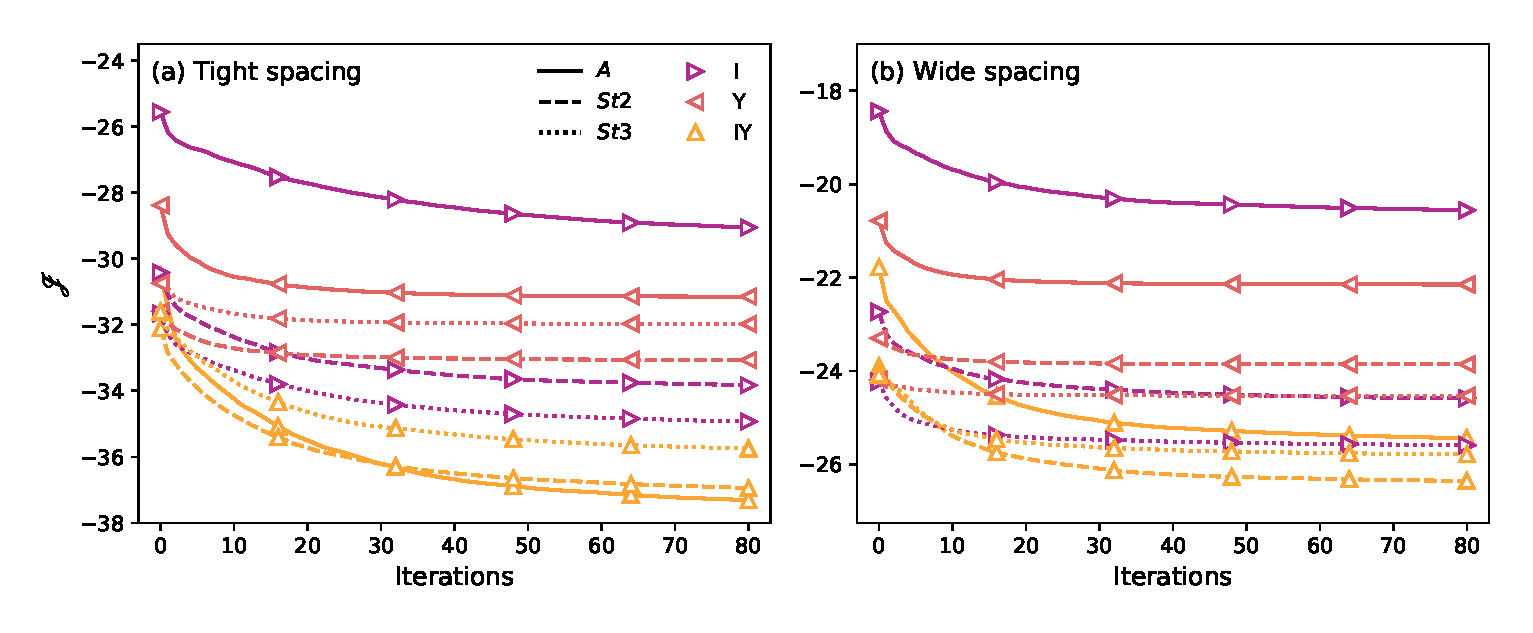
\includegraphics[width=\textwidth]{Torque18/convergence.eps}
	\caption{Cost functional decrease in terms of BFGS iterations for all optimization cases in window 6. (a) Tight spacing optimal control cases. (b) Wide spacing optimal control cases. Linestyles indicate the wind-farm layout. Markers (plotted every 15 iterations) indicate the control case.\label{fig:convergence} }
\end{figure}

\subsection{Power Extraction and Wind-Farm Efficiency}

Figure \ref{fig:wf_effic} and Table \ref{tab:efficiency_numerical_vals} show the wind-farm efficiency for all simulation cases. A first observation is that the optimal control approach achieves significant power gains in every case except for case Y in St3$_W$. The latter can be explained by the fact that the St3$_W$ layout already has a relatively high reference efficiency due to its large streamwise turbine spacing and that the turbine placement leaves limited room for increasing power through wake redirection. Furthermore, the improvements in wind-farm efficiency are higher for wind farms with more severe axial wake interactions, i.e. higher for aligned than for staggered layouts, and higher for tight than for wide spacings. Note also that optimal control allows the turbine density to be increased significantly without sacrificing too much efficiency: for example, case IY of layout A$_T$ achieves an efficiency close to the reference case of St2$_W$, but using only 36$\%$ of the surface area per turbine of the latter. 

For all layouts except St3$_W$, the combined yaw and induction controls in case IY significantly outperform separate yaw and induction controls of cases Y and I respectively. Interestingly, when comparing the merits of yaw and induction control, the control strategy with the highest yield is dependent on the wind-farm layout: for aligned wind farms A$_T$ and A$_W$ yaw control allows to achieve higher power extraction than induction control (consistent with the observations by Munters and Meyers \cite{muntersenergies}), whereas for all staggered cases induction control is slightly more advantageous than yaw control. This shows that the most advantageous control strategy depends on the effective layout of the wind farm, which in turn depends on the mean wind direction, and hence justifies further research into both control strategies.  

\begin{figure}
	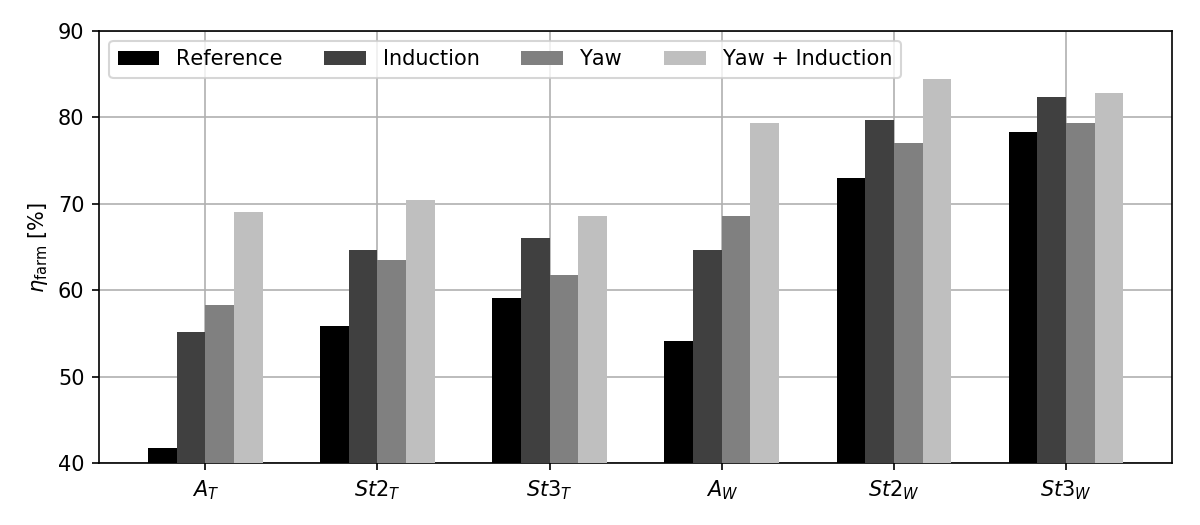
\includegraphics[width=\textwidth]{Torque18/power_gain_bar}
	\caption{Wind-farm efficiency $\eta_{\rm farm}$ with respect to a reference case in which every turbine produces the average power of the first-row turbines in the $A_T$ layout. Errorbars indicate confidence intervals of $\pm$ 2 standard deviations and are calculated using the procedure detailed in Appendix C of Ref. \cite{muntersenergies}. \label
		{fig:wf_effic}}
\end{figure}

\begin{table}
\centering
\caption{Wind-farm efficiencies for all simulation cases, including the relative increase over the greedy reference control cases in brackets. \label{tab:efficiency_numerical_vals}}
\begin{tabular}{rcccccc}
	\hline 
				  & & Tight  & & & Wide & \\ 
			   	     & $A$ 	& $St2$  & $St3$ & $A$ & $St2$  & $St3$ \\ 
	\hline 
	R  & 0.42	    & 0.56	     & 0.59	         & 0.54	         & 0.73	      & 0.78	\\ 
	I  & 0.54 [+31\%] & 0.65 [+16\%] & 0.66   [+12\%]  & 0.65 [+20\%]    & 0.80 [+9\%]  & 0.82 [+5\%]\\ 
	Y  & 0.59 [+39\%] & 0.64 [+14\%] & 0.62	[+4\%]     & 0.68 [+26\%]   & 0.77 [+6\%]  & 0.79 [+1\%]\\ 
	IY & 0.70 [+66\%] & 0.71 [+26\%] & 0.69	[+16\%]    & 0.79 [+46\%]    & 0.84 [+15\%] & 0.82 [+6\%]\\ 
	\hline 
\end{tabular} 
\end{table}

Row-averaged power extraction is shown in Fig. \ref{fig:power_row}. Panels (a) and (d) illustrate the tightly spaced and widely spaced aligned layouts respectively, for which is was found that yaw control was more favorable than induction control. It is shown that first-row power is curtailed more for cases Y and IY (involving yaw control) than for case I based on induction, and more so for a tight than for wide turbine spacings, consistent with larger yaw misalignments required to redirect wakes over shorter distances (see further below). Power extraction in downstream rows is in the same range for yaw and induction control, with yaw control achieving higher gains than induction control. The power extraction for the two-row staggered St2 layout in panels (b) and (e) shows power gains for yaw and induction control to lie much closer together throughout the entire wind farm, with a slight advantage for induction control, especially in rows 3 and 4 of the widely spaced layout. Panels (c) and (f) illustrate that, for the three-row staggered St3 layout it is more difficult to significantly increase power extraction over the greedy reference case, with relatively limited gains for induction control and even smaller ones for yaw control. 

\begin{figure}
	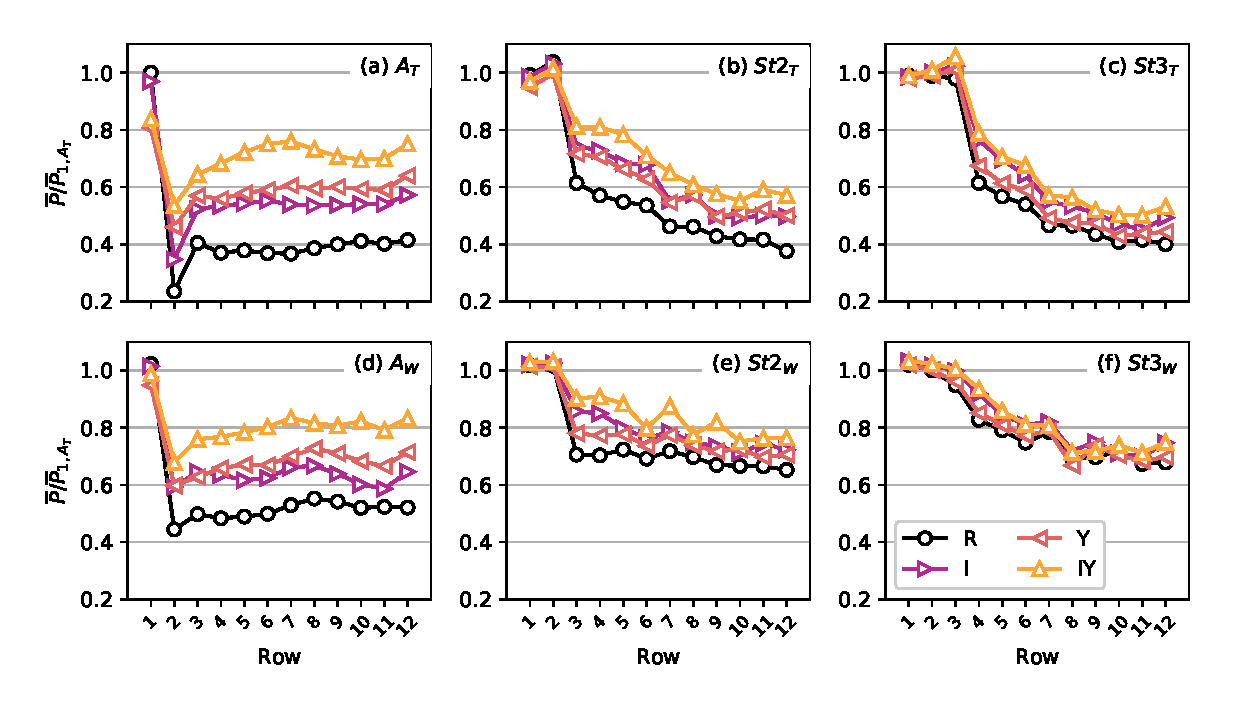
\includegraphics[width=\textwidth]{Torque18/power_row}
	\caption{Row-averaged mean power extraction for all simulation cases, normalized by first-row mean power in the reference case of the $A_T$ layout.\label{fig:power_row}}
\end{figure}



\subsection{Time-averaged Flow Field}
The current section discusses the time-averaged flow field of the different control cases. For brevity and clarity of the discussion, we omit the three-row staggered St3 layout and focus on the aligned A and two-row staggered St2 layout, which exhibit a much larger increase in performance for the optimal control cases. 


Firstly, we provide a qualitative illustration of how the optimized controls influence the wind-farm flow field. Figures \ref{fig:ax_tight} and
\ref{fig:ax_wide} show contours of the time-averaged axial velocity at hub height for the tightly and widely spaced wind farms respectively. For
clarity of representation, only a selected amount of wind turbine columns are shown. We first discuss the tightly spaced wind farms in Fig.
\ref{fig:ax_tight}. The figure shows that, in the reference control case R, wakes propagate with the mean wind direction, resulting in reduced disk velocities for downstream turbines. Furthermore, it is shown that wakes expand and
recover as they propagate downstream, and that the staggered layout allows wakes to recover over a larger streamwise length, corresponding to the
larger baseline efficiency as observed above. For the induction control cases (I), the overall flow fields look qualitatively similar, both for the
aligned and the staggered layout, although close inspection shows slightly higher disk velocities for downstream turbines originating from increased wake mixing, associated with the power
gains discussed above. Turning to the yaw control simulation (Y), it can be seen that, for the aligned case, turbines redirect wakes away from their
downstream neighbors by misaligning their yaw angles with the incoming flow. Furthermore, the distribution of mean yaw angles throughout the farm
seems quite orderly: turbines within the same column seem to adhere to similar yaw angles (note that, due to the time averaging, effects of dynamic
yaw are not visbile in the current representation). For the staggered layout, wakes are also deflected away from downstream turbines, although yaw
angles are overall smaller throughout the farm, and the distribution of mean yaw angles is less ordered than for the aligned case. The same
observations are made for the induction--yaw cases (IY), for which the flow fields appear very similar ot the yaw control cases.

\begin{figure}[t]
	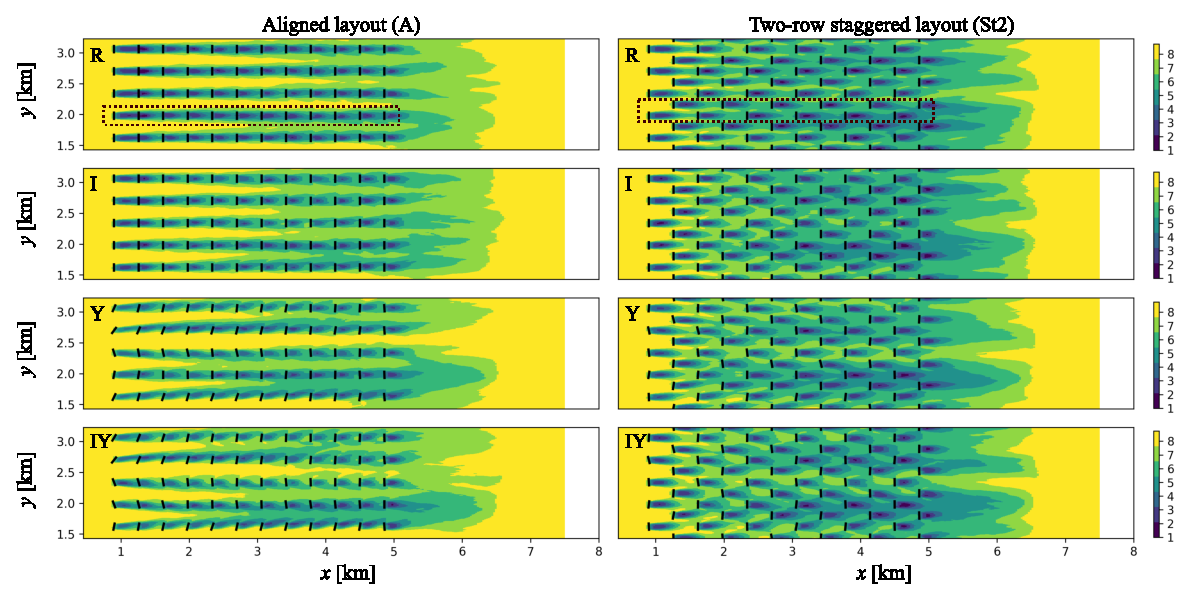
\includegraphics[width=\textwidth]{Torque18/tight_stat}
	\caption{Contours of axial velocity at hub height for tightly-spaced wind farms. Turbine rotors are yawed according to the time-averaged turbine yaw angle. \emph{Left: } Aligned layout. \emph{Right: } Two-row staggered layout. \emph{From top to bottom:} Greedy reference control (R), Induction control (I), Yaw control (Y), Combined yaw and induction control (IY). Coloring is in units of m s$^{-1}$. Dotted rectangles in the top panels indicate turbines for which yaw and thrust coefficients are plotted in Figs. \ref{fig:yaw} and \ref{fig:ctfilt}. \label{fig:ax_tight}}
\end{figure}

Moving on to the widely-spaced farms in Fig. \ref{fig:ax_wide}, the same story can largely be retold. The flow fields of the induction control cases closely resemble the reference flow, with slightly higher axial velocities at the downstream turbine disk. Flow fields for yaw control and combined induction--yaw control again appear similar.  For the aligned layout, wakes are clearly being deflected away from downstream turbines. Note however that the mean yaw angles are smaller than those in the tightly spaced wind farms, due to the fact that a larger streamwise spacing allows wakes to be deflected at smaller angles while still missing downstream turbines. For the staggered layout, wake deflection is not clearly visible in the time-averaged flow fields discussed here. 


\begin{figure}[t]
	\includegraphics[width=\textwidth]{Torque18/wide_stat}
	\caption{Contours of axial velocity at hub height for widely-spaced wind farms. Turbine rotors are yawed according to the time-averaged turbine yaw angle. \emph{Left: } Aligned layout. \emph{Right: } Two-row staggered layout. \emph{From top to bottom:} Greedy reference control (R), Induction control (I), Yaw control (Y), Combined yaw and induction control (IY). Coloring is in units of m s$^{-1}$. Dotted rectangles in the top panels indicate turbines for which yaw and thrust coefficients are plotted in Figs. \ref{fig:yaw} and \ref{fig:ctfilt}. \label{fig:ax_wide}}	
\end{figure}

\subsection{Control Dynamics}
The current section provides a qualitative impression of the control dynamics for a selected set of turbines, i.e. the turbine column at $y \approx 2$ km (see Fig. \ref{fig:ax_tight},\ref{fig:ax_wide}). The overall goal of the current section is to illustrate general patterns in the control signals. A more quantitative analysis of the controls is outside the scope of the current paper. 

Figure \ref{fig:yaw} shows a space-time plot of yaw angles for all cases involving yaw control, i.e. case Y and IY for staggered and aligned layouts, and tight and wide spacings. The dashed lines indicate the advection time between aligned rows, and the dotted lines indicate the advection time between staggered rows. From the figure, several characteristics of the yaw behavior can be observed. First, it can be seen that the yaw dynamics for exclusive yaw control and combined induction--yaw control are very similar. Next, maximum yaw deviations are shown to be larger for the aligned layouts than for their staggered counterparts, and larger for tight spacings than for wide spacings. Also, for the tight aligned layout, it is shown that the first turbine row adjusts its yaw angle dynamically in response to incoming flow conditions, whereas the yaw angle of downstream turbines follows suit after the advection time between turbine rows. This effect can also be seen for the wide aligned layout and, to a lesser extent, for the tight staggered layout, in which the advection time is somewhat more complicated due to the staggering of subsequent rows. The yaw behavior of the wide staggered layout is more disorderly. Yaw characteristics for the other columns are similar, although some columns turn to a relatively stable yaw misalignment early on in the simulation and do not exhibit significant dynamics afterwards (e.g. the column at $y = 1.5$ km, see Figs. \ref{fig:ax_tight}, \ref{fig:ax_wide}, not further shown here).

\begin{figure}[t]
	\centering
	\includegraphics[width=0.9\textwidth]{Torque18/yaw_angles}
	\caption{Space-time plot of yaw angles in turbine column at $y \approx $ 2 km for yawing control cases I and IY, i.e. every horizontal color data represents yaw angle time series for a single turbine. Dashed (dotted) lines indicate the advection time between aligned (staggered) rows. Coloring is in units of degrees. \label{fig:yaw}}
\end{figure}

Space-time plots for the thrust coefficients in cases I and IY are shown in Fig. \ref{fig:ctfilt} (for the same turbines as in Fig. \ref{fig:yaw}). In contrast to the yaw angles discussed previously, for the thrust coefficients no clear patterns can be observed qualitatively. A general observation is that variations and reductions in $\cthat$ are apparent more in aligned cases than their staggered counterparts, and more in tight spacings than in wide spacings. Also, the combined induction--yaw IY cases tend to higher values of $\cthat$ than the exclusive induction control cases. 

\begin{figure}[b]
	\centering
	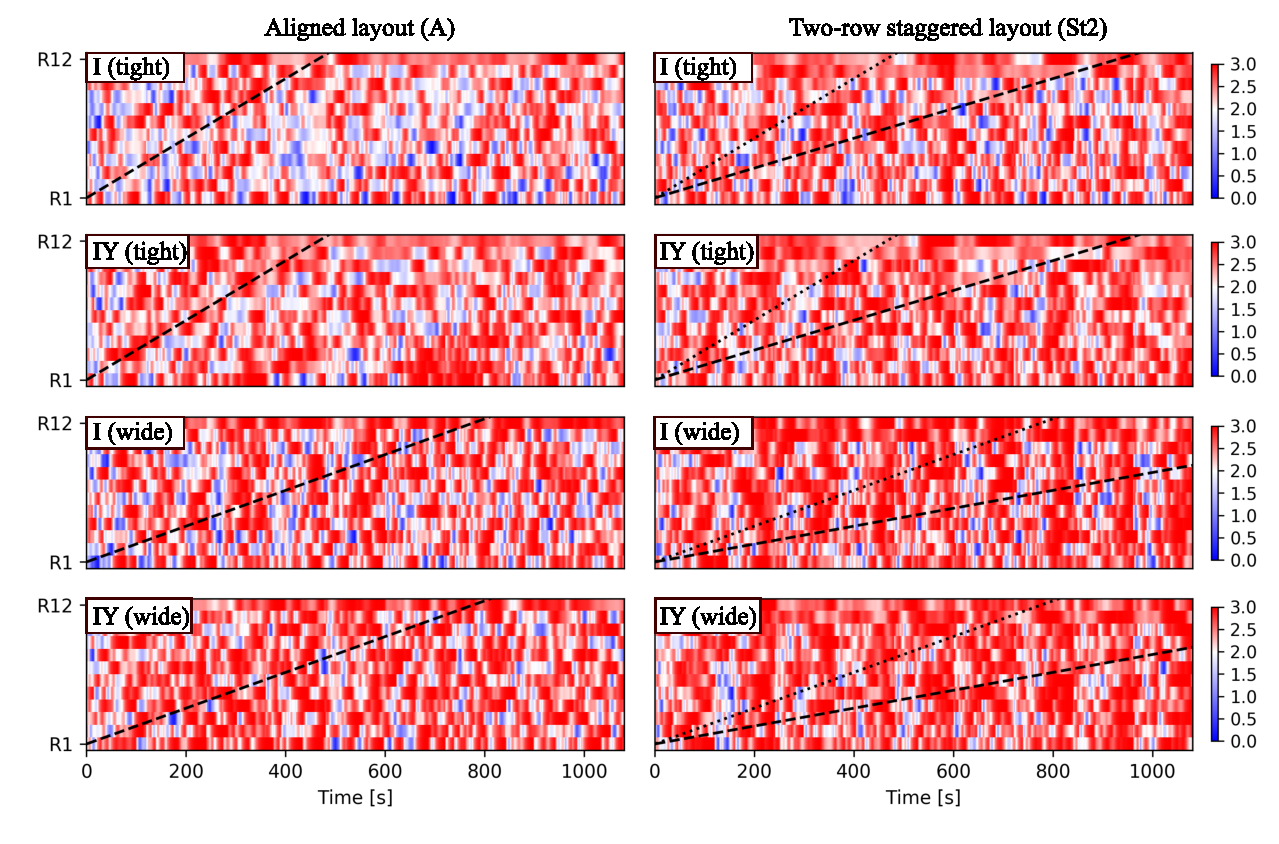
\includegraphics[width=0.9\textwidth]{Torque18/ctfilts}
	\caption{Space-time plot of thrust coefficients in turbine column at $y \approx $ 2 km for yawing control cases I and IY, i.e. every horizontal color data represents yaw angle time series for a single turbine. Dashed (dotted) lines indicate the advection time between aligned (staggered) turbines. \label{fig:ctfilt}}
\end{figure}




\section{Conclusion}\label{sec:conc}
The current study performed optimal induction and yaw control for a set of aligned and staggered wind farms with varying spacing with the aim of quantifying potential power gains in different wind-farm setups and investigating the utility of yaw and induction in large-scale wind farms. The optimal control simulations indicated that, for virtually all cases, both induction and yaw control lead to a significant increase in wind-farm efficiency. Furthermore it was found that, using optimal coordinated control, turbine density can be increased without significant sacrifice of farm efficiency, i.e. the combined induction--yaw control of the tightly spaced aligned farm approximates the reference efficiency of the widely spaced staggered farm. Also, simulations show that the most promising control strategy of exclusive yaw and induction control depends on the wind-farm layout, and hence on the mean wind direction in practice, with aligned layouts favoring yaw control and staggered layouts slightly favoring induction control. 

A qualitative investigation of flow field characteristics and control dynamics show that, for aligned wind-farm layouts, induction control leads to increased wake mixing whereas yaw control is used for wake redirection. The time-averaged flow field over combined induction--yaw control closely resembles that of yaw control. Results for the staggered layouts show no significant deviations from the reference case from a qualitative perspective. For the yaw dynamics it was found that the first-row turbine takes the lead and reacts to incoming flow variations by dynamically changing its yaw angle, whereas downstream turbines follow suit of their upstream neighbors after the wake advection time. Thrust coefficient dynamics are much more complex and were not further investigated. 

Some remarks have to be made upon interpretation of the current results. Firstly, the fact that the optimization horizon $T$ covers only an advection time of about 4 rows of the widely spaced farm instead of an entire wind farm flow-through tends to allow more interaction between turbines in wind farms with small axial distances between turbines. This could possibly lead to higher gains in aligned versus staggered layouts, and in tightly versus widely spaced farms. On the other hand, turbulent flows are due to their chaotic nature by definition harder to control over longer distances, which would complicate control over longer distances anyway in practice. In order to fully quantify these effects, the optimization horizon should be enlarged. However, the adjoint method fails for control of chaotic systems over longer time horizons, and hence an alternative such as the least-squares shadowing approach should be used \commwim{ADDREF}. Furthermore, due to the nonconvexity of the optimization problem at hand, the optimal controls from the current simulations are most probably local optima. A complete comparison between the merits of different control strategies would require a global optimization to be performed. However, such optimizations are infeasible given current computational resources, and we experience that the optimized cost functional value is largely unaffected by the specific local optimum to which the algorithm converges \cite{munters}. 

\section*{Acknowledgements}
The authors acknowledge funding by the European Research Council (ActiveWindFarms, grant no. 306471). The computational resources and services used in this work were provided by the VSC (Flemish Supercomputer Center), funded by the Research Foundation Flanders (FWO) and the Flemish Government department EWI. 

%\section*{References}
%\bibliography{\begin{thebibliography}{9}
%		\bibitem{nilsson2014large} Nilsson K, Ivanell S, Hansen K S, Mikkelsen R, S\o rensen J N, Breton S-P, Henningson D 2014 Large-eddy simulations of the Lillgrund wind farm {\it Wind Energy} {\bf 18}, pp. 449 -- 467
%		
%		\bibitem{annoni2015analysis} Annoni J, Gebraad P, Scholbrock A K, Fleming P A, van Wingerden J-W 2015 Analysis of axial-induction-based wind plant control using an engineering and a high-order wind plant model {\it Wind Energy} {\bf In press}	
%		
%		\bibitem{goit2015optimal} Goit J P and Meyers J 2015 Optimal control of energy extraction in wind-farm boundary layers {\it J Fluid Mech} {\bf 768} pp. 5--50
%		
%		\bibitem{goit2016optimal} Goit J P, Munters W and Meyers J 2016 Optimal Coordinated Control of Power Extraction in LES of a Wind Farm with Entrance Effects {\it Energies} {\bf 9}, 29
%		
%		
%%	\bibitem{goit} J. P. Goit, J. Meyers 2015, Optimal control of energy extraction in wind-farm boundary layers, J Fluid Mech 768, 5--50
%%%	\bibitem{munters} W. Munters, J. Meyers 2017, 'An optimal control framework for dynamic induction control of wind farms and their interaction with the atmospheric boundary layer', Phil Trans R Soc A 375, 20160100
%%%	\bibitem{phd} W. Munters, 'Large eddy simulations and optimal coordinated control of wind-farm boundary layers', PhD Thesis, KU Leuven, December 2017
%\end{thebibliography}


\section*{References}
\begin{thebibliography}{9}
	\bibitem{goit} J. P. Goit, J. Meyers 2015, `Optimal control of energy extraction in wind-farm boundary layers', J Fluid Mech 768, 5--50
	\bibitem{munters} W. Munters, J. Meyers 2017, `An optimal control framework for dynamic induction control of wind farms and their interaction with the atmospheric boundary layer', Phil Trans R Soc A 375, 20160100
	\bibitem{munterswes} W. Munters, J. Meyers 2018, `Towards practical dynamic induction control of wind farms: analysis of optimally controlled wind-farm boundary layers and sinusoidal induction control of first-row turbines', Wind Energ. Sci. Discuss., in review, 2018. 
	\bibitem{muntersenergies} W. Munters, J. Meyers 2018, `Dynamic Strategies for Yaw and Induction Control of Wind Farms Based on Large-Eddy Simulation and Optimization', Energies 11(1), 177
	\bibitem{byrd} H. R. Byrd, , P. Lu, J. Nocedal, C. Zhu 1995. `A limited memory algorithm for bound constrained optimization.' SIAM Journal on Scientific Computing 16(5), 1190-1208
\end{thebibliography}

\end{document}


